\documentclass{jarticle}
\usepackage[dvipdfmx]{graphicx}

\newcommand*{\mbold}[1]{\mbox{\boldmath $#1$}}
\newcommand*{\doubleint}{\int\!\!\!\int}
\newcommand*{\trippleint}{\int\!\!\!\int\!\!\!\int}

\begin{document}

\section{}
\subsection{}
\subsection{}
Conservertive force : 
\begin{equation}\label{eq:conv_force}
	F_i = -\frac{\partial V}{\partial x_i}, ~~~~ V : scalar
\end{equation}

\subsubsection*{(a) Pysics of the sun and the earth}

Modeling :
\begin{itemize}
\item Mass of the sun $M$ is much larger than mass of the earth $m$, so,  we consider the sun is fixed to the origin of the inertial system. 
\item Diameter of the sun(1400,000km) and that of the earth(6400km) is much smaller than the distance between the sun and the earth(150000000km), so, we consider them as mass points.
\end{itemize}

Universal gravitaion force : 
\begin{equation}
	F_i = -G\frac{mM}{R^2}\frac{x_i}{R}
\end{equation}

Using eq(\ref{eq:conv_force}), 
\begin{equation}\label{eq:diff_eq}
	\frac{\partial V}{\partial x_i} = G\frac{mM}{R^2}\frac{x_i}{R} .
\end{equation}

$V$ is a function of $\{x_i\}_{i=1}^3$, then,
\[
	dV = \sum_{i=1}^3 \frac{\partial V}{\partial x_i} dx_i .
\]

Using eq(\ref{eq:diff_eq}), 
\[
	dV = GmM \sum_{i=1}^3 \frac{x_i}{R^3} dx_i = GmM \frac{\mbold{R}}{R^3}\cdot d\mbold{R}
\]

$d\mbold{R}$ is composed by the component parallel with $\mbold{R}$ and the component perpendicular with $\mbold{R}$, 
\[
	d\mbold{R} \equiv d\mbold{R}_\perp +d \mbold{R}_\parallel
\]

$\mbold{R} \cdot d\mbold{R}_\perp = 0$, then, 
\[
	dV = GmM\frac{\mbold{R}}{R^3} \cdot d\mbold{R}_\parallel = GmM\frac{1}{R^2}dR_\parallel
\]

$dR_\parallel$ is the small change of $R$, so, it can be written as $dR$. 

\[
	dV = GmM\frac{dR}{R^2}
\]

Thus, 

\[
	V = -GmM\frac{1}{R}
\]

\subsubsection*{(b) Physics of the earth and the satellite}

Modeling : 
\begin{itemize}
\item Mass of the earth $M$ is much larger than mass of the satellite $m$, so,  we consider the earth is fixed to the origin of the inertial system. 
\item The height of the satellite orbit(over 100km) is much larger than the size of satellite, so we consider the satellite as a mass point.
\item The earth is the aggregation of many($N$) small mass($m_i$). Any small mass is fixed to each position by all the other small mass.
\end{itemize}

We can choose the size of small mass so that (the size of satellite) $\ll$ (the distance between the satellite and the small mass).
Then, the situation is same as (a). The universal gravitation acting on the satellite is, 

\[
	\mbold{F} = -\sum_{i=1}^N \frac{G m m_i}{R_i^2}\frac{\mbold{R_i}}{R_i}
\]

By the same calcuration as (a), 
\[
	V = -\sum_{i=1}^N \frac{G m m_i}{R_i}
\]

\subsection{}
The density of the earth : 
\begin{equation}
	V(x,y,z) = -Gm \trippleint \frac{dx^\prime dy^\prime dz^\prime \rho(x^\prime, y^\prime, z^\prime)}{\sqrt{(x - x^\prime)^2 + (y - y^\prime)^2 + (z - z^\prime)^2}}
\end{equation}

\subsubsection*{(a) Perfect sphere, constant density}
$\rho = const$, then
\begin{equation}\label{eq:const_dens_potential}
	V(x,y,z) = -Gm\rho \trippleint \frac{dx^\prime dy^\prime dz^\prime}{\sqrt{(x - x^\prime)^2 + (y - y^\prime)^2 + (z - z^\prime)^2}}
\end{equation}

Consider polar system : 
\begin{figure}[htbp]
	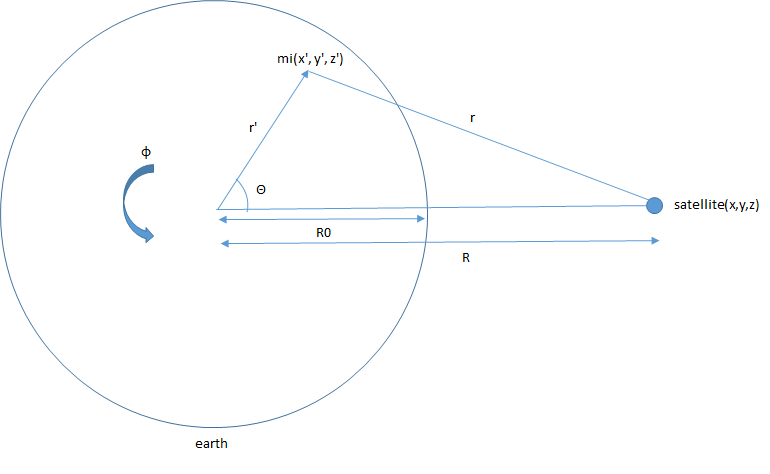
\includegraphics[width=10cm]{earth_satellite.png}
\end{figure}

On the polar system$(r^\prime, \theta, \phi)$ whose origin is the centre of the earth, the distance between the satellite and the small mass $m_i$ is, 
\begin{equation}
	r = \sqrt{r^{\prime 2} + R^2 - 2 r^\prime R \cos\theta}
\end{equation}

Jacobian is $r^{\prime 2}\sin\theta$, then
\begin{equation}
	dx^\prime dy^\prime dz^\prime = r^{\prime 2}\sin\theta drd\theta d\phi
\end{equation}

In the perfect sphere, $0 \leq r^\prime \leq R_0$, $0 \leq \theta \leq \pi$, and $0 \leq \phi \leq 2\pi$, then,  eq(\ref{eq:const_dens_potential}) can be calcurated, 
\begin{eqnarray}\label{eq:calcurated_potential}
	&&-Gm\rho \trippleint \frac{dx^\prime dy^\prime dz^\prime}{\sqrt{(x - x^\prime)^2 + (y - y^\prime)^2 + (z - z^\prime)^2}} \nonumber \\	 
	&&= -Gm\rho \int_0^{2\pi} d\phi \int_0^{R_0} dr^\prime \int_0^\pi d\theta \frac{r^{\prime 2}\sin\theta}{\sqrt{r^{\prime 2} + R^2 - 2 r^\prime R \cos\theta}} \nonumber \\	
	&&= -2\pi Gm\rho \int_0^{R_0} dr^\prime \int_{-1}^{1} \frac{-r^{\prime 2} d(\cos\theta)}{\sqrt{r^{\prime 2} + R^2 - 2 r^\prime R \cos\theta}} \nonumber\\
	&&= -2\pi Gm\rho \int_0^{R_0} dr^\prime \left[ \frac{-2r^{\prime 2} \sqrt{r^{\prime 2} + R^2 - 2 r^\prime R \cos\theta}}{-2r^\prime R} \right]_{\cos\theta = -1}^{\cos\theta = 1} \nonumber \\
	&&= \frac{2\pi Gm\rho}{R} \int_0^{R_0} dr^\prime r^\prime (|r^\prime - R| - (r^\prime + R)) 
\end{eqnarray}

The satellite is outside of the earth, then $R > R_0 \Rightarrow r^\prime < R$, eq(\ref{eq:calcurated_potential}) becomes,
\begin{equation}
	-\frac{2\pi Gm\rho}{R} \int_0^{R_0} dr^\prime 2r^{\prime 2} = -\frac{Gm}{R}\frac{4\pi R_0^3}{3}\rho = -\frac{GmM}{R}
\end{equation}

Considering the case $R < R_0$, we can calcurate the potential inside the earth. 
Eq(\ref{eq:calcurated_potential}) becomes,
\begin{eqnarray}
	V &=& \frac{2\pi Gm\rho}{R} \left[ \int_0^R dr^\prime r^\prime (-2r^\prime) + \int_R^{R_0} dr^\prime r^\prime (-2R) \right] \nonumber \\
	&=& \frac{2\pi \rho mG}{3}R^2 - 2\pi G m\rho R_0^2
\end{eqnarray}

The force is,
\begin{equation}
	\mbold{F} = -\nabla V = -\frac{2\pi \rho m G}{3}\nabla (R^2)
\end{equation} 

Using, 
\[
	(\nabla (R^2))_i = \frac{\partial}{\partial x_i}\sum_{j=1}^3 x_j^2 = 2x_i
\]

\begin{equation}
	\mbold{F} = -\frac{4\pi \rho m G}{3}\mbold{R}
\end{equation}

$\mbold{F}$ is a harmonic oscillator force. Potential has a form as $aR^2 +b$. Harmonic oscillator potential.

Simulated result is following.
\begin{figure}[htbp]
	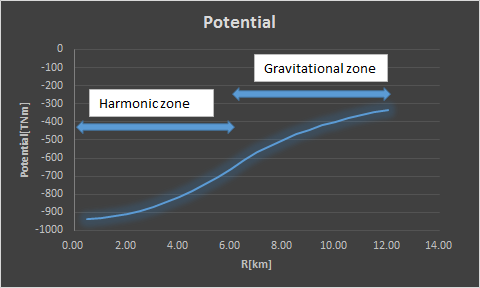
\includegraphics[width=10cm]{potential_plot.png}
\end{figure}
\begin{figure}[htbp]
	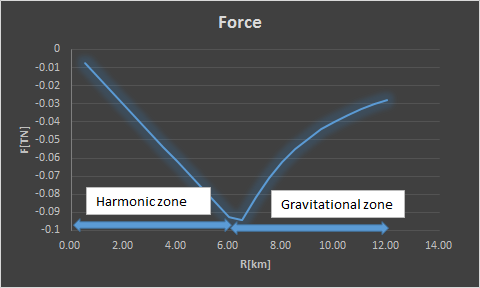
\includegraphics[width=10cm]{force_plot.png}
\end{figure}

\subsubsection*{(b) Effect of small distortion from sphere} 

To be accurate, the earth is not a perfect shpere. So, the area to be integrated in eq(\ref{eq:calcurated_potential}) should be corrected. But, the volme of the area to be added or removed is much smaller than the earth diameter. For example, the deepest point of the sea, the Mariana Trench is 10000m depth. Another example, highest mountain Evelest is 8800m height. 
We consider that the 


\end{document}